\documentclass[main]{subfiles}


\begin{document}
	\begin{lect} {2019-09-30}
		\section{Дифференциальная геометрия поверхностей}
		\subsection{Понятие поверхности}
		\begin{example}[способы задания поверхностей]
			\begin{enumerate}
				\item $z=f(x,y)$ - явное задание
				\item $F(x,y,z)=0$ - неявное задание
			\end{enumerate}
		\end{example}

		\begin{Theorem}[о неявной функции]
			\[F(x,y,z)=0,\q F \text{ - непр. дифф.},\q F(x_0,y_0,z_0)=0,\q \dfrac{\d f}{\d z}\big|_{(x_0,y_0,z_0)} \neq 0\]
			\[\Ra \e f(x,y): F(x,y,f(x,y))=0 \text{ в некоторой окр.}\]
		\end{Theorem}

		\begin{Definition}
			\[D \subset \R^2,\q \forall (u,v) \in D,\q \ol{r} - \text{инъекция}\]
            \[\begin{cases}
				x=x(u,v)\\
				y=y(u,v)\\
				z=z(u,v)
			\end{cases}\]
			\[\ol{r}=\ol{r}(u,v)\q \ol{r}: D \ra \R^3\]
		\end{Definition}

		\begin{Example}
			\[z=f(x,y)\]
			\[\begin{cases}
				x=u\\
				y=v\\
				z=f(u,v)
			\end{cases}\] \\
			Координат. линии поверхности:
			\[u=u_0\q \ol{r}(u,v) \text{ - кривая}\]
			\[\ol{r}(u,v) \text{ - другое семейство}\]
		\end{Example}

		\begin{remark}
			Линии перпендикулярны
		\end{remark}

		\begin{definition}
			Перепараметризация - биекция
			\begin{figure}[H]
			    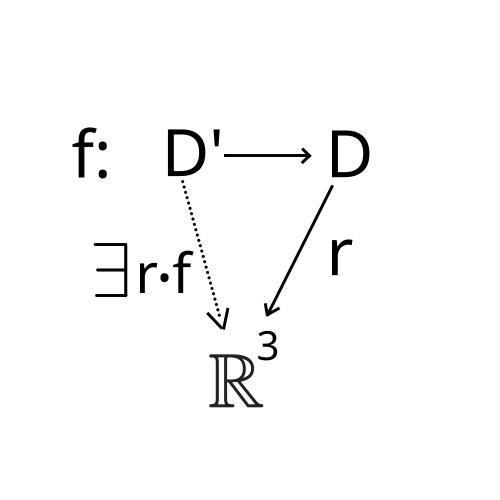
\includegraphics[width=4cm]{pics/5_2.png}
			    \centering
			\end{figure}
		\end{definition}

		\begin{definition}
			Параметризация называется регулярной, если
			\[\dfrac{\d \ol{r}}{\d u} \text{ и } \dfrac{\d \ol{r}}{\d v} \text{ не перпендикулярны ни в одной точке}\]
			\[(\lra \dfrac{\d \ol{r}}{\d u} \times \dfrac{\d \ol{r}}{\d v} \neq 0)\]
		\end{definition}

		\begin{definition}
			Кривая лежит на поверхности, если все её точки лежат на поверхности\\
		    \[\begin{cases}
				u = u(t)\\
				v = v(t)
			\end{cases}\]
			\[\Ra \ol{r}=(x(u(t), v(t)),\ y(...)...)\]
		\end{definition}

		\begin{definition}
			Вектор называется касательным, если он является касательным к кривой на поверхности
		\end{definition}

		\begin{theorem}
			Если поверхность регулярная $\Ra$ касательные векторы образуют плоскость
		\end{theorem}

		\hsubsection{2.2}{Касательная плоскость}
		\begin{definition}
			Касательная плоскость - плоскость из касательных векторов
		\end{definition}

		\begin{proof}
			Базис: $\dfrac{\d r}{\d u} \bigg|_A$ и $\dfrac{\d r}{\d v} \bigg|_A$\\
            \[\begin{cases}
				u=t\\
				v=v_0
			\end{cases}\]
			\[\begin{cases}
				u^2 = u_0\\
				v=t
			\end{cases}\]
			\[\ol{r}(t) = (x(t_0,v_0),\ y(t_0,v_0),\ z(t_0,v_0))\]
			\[\ol{r'}(t) = \Br{x'(t_0,v_0),\ y'(t_0,v_0),\ z'(t_0,v_0)} = \Br{\dfrac{\d x}{\d u}...}\]

			\[u=u(t)\]
			\[v=v(t)\]
			\[\dfrac{d r}{d t} \Big|_A = \Br{\dfrac{\d \ol{r}}{\d u}} \dfrac{d u}{d t} + \dfrac{\d \ol{r}}{\d v} \dfrac{d v}{d t}} \Big|_A\]
			Наоборот $\alpha \dfrac{\d \ol{r}}{\d u} \Big|_A + \beta \dfrac{\d \ol{r}}{\d v} \Big|_A$ - вектор\\
			\[\begin{cases}
				u(t) = \alpha t\\
				v(t) = \beta t
			\end{cases}\]
		\end{proof}

		Как задать касательную плоскость в координатах?\\
		Пусть $\ol{n}$ - нормаль к плоскости
		\[\ol{n} = (A,\ B,\ C)\]
		\[\Ra A(x-x_0)+B(y-y_0)+C(z-z_0)=0\]
		\[\ol{n} = \dfrac{\d \ol{r}}{\d u} \times \dfrac{\d \ol{r}}{\d v}\]
		\[\ol{r} = (x,\ y,\ z)\]
		\[\dfrac{\d \ol{r}}{\d u} = \Br{\dfrac{\d x}{\d u},\ \dfrac{\d y}{\d u},\ \dfrac{\d z}{\d u}}\]
		\[\dfrac{\d \ol{r}}{\d v} = \Br{\dfrac{\d x}{\d v},\ \dfrac{\d y}{\d v},\ \dfrac{\d z}{\d u}}\]
		\[\ol{n} = \begin{pmatrix}
			\begin{vmatrix}
				\dfrac{\d y}{\d u} & \dfrac{\d z}{\d u}\\ \\
				\dfrac{\d y}{\d v} & \dfrac{\d z}{\d v}
			\end{vmatrix},\
			\begin{vmatrix}
				\dfrac{\d z}{\d u} & \dfrac{\d x}{\d u}\\ \\
				\dfrac{\d z}{\d v} & \dfrac{\d x}{\d v}
			\end{vmatrix},\
			\begin{vmatrix}
				\dfrac{\d x}{\d u} & \dfrac{\d y}{\d u}\\ \\
				\dfrac{\d x}{\d v} & \dfrac{\d y}{\d v}
			\end{vmatrix}
		\end{pmatrix}\]
		\[\Ra \det \begin{vmatrix}
			\dfrac{\d x}{\d u} & \dfrac{\d y}{\d u} & \dfrac{\d z}{\d u}\\ \\
			\dfrac{\d x}{\d v} & \dfrac{\d y}{\d v} & \dfrac{\d z}{\d v}\\ \\
			x-x_0 & y-y_0 & z-z_0
		\end{vmatrix} = 0 \text{ - уравнение касательной плоскости}\]

		\begin{utv}
			В неявном виде
			\[\nabla F = \Br{\dfrac{\d F}{\d x},\ \dfrac{\d F}{\d y},\ \dfrac{\d F}{\d z}} \text{ - перп. плоскости}\]
			\[\begin{cases}
				x=x(t)\\
				y=y(t)\\
				z=z(t)
			\end{cases}\]
			\[\dfrac{d F}{d t} = 0 \q \dfrac{d F}{d t} = \dfrac{\d F}{\d x} \dfrac{d x}{d t} + \dfrac{\d F}{\d y} \dfrac{d y}{d t} + \dfrac{\d F}{\d z} \dfrac{d z}{d t} = \nabla F \circ \us{\text{касат. вектор}}{(x',y',z')}=0\]
			\[\nabla F \bot \text{касат. вектору (любому)} \Ra \nabla F \text{ - норм пов-ть}\]
		\end{utv}

		\begin{utv}
				Уравнение касательной плоскости:
				\[\dfrac{\d F}{\d x}(x-x_0) + \dfrac{\d F}{\d y}(y-y_0) + \dfrac{\d F}{\d z}(z-z_0)\]
		\end{utv}

		\subsection{Первая квадратичная форма}
		\[\begin{cases}
			u=u(t)\\
			v=v(t)
		\end{cases}\]
		$\ol{r}$ - пов-ть
		\[r=(x,y,z)=(x(u(t),v(t)),\ y(u(t),v(t)),\ z(u(t),v(t)))\] %разбить на строки


        \begin{multline*}
            \text{Длина кривой} = \int_{t_0}^{t_1} \abs{\dfrac{d}{dt} \ol{r} (u(t), v(t))} dt =\\
            =\int_{t_0}^{t_1} \abs{\Br{
			    \dfrac{\d x}{\d u}u' + \dfrac{\d x}{\d v}v', \
		    	\dfrac{\d y}{\d u}u' + \dfrac{\d y}{\d v}v', \
			    \dfrac{\d z}{\d u}u' + \dfrac{\d z}{\d v}v'
	    	}} dt =\\
            =\int_{t_0}^{t_1}
		    	\sqrt{\dfrac{\d x}{\d u}^2 u'^2 + 2\dfrac{\d x}{\d u} \dfrac{\d x}{\d v}u'v' + \dfrac{\d x}{\d u}^2 v'^2 + ...
                		} \ dt =\\
		= \int_{t_0}^{t_1} \sqrt{
			E u'^2 + 2 F u' v' + G v'^2
		} dt
        \end{multline*}

		\[E = \Br{\dfrac{\d x}{\d u}}^2 + \Br{\dfrac{\d y}{\d u}}^2 + \Br{\dfrac{\d z}{\d u}}^2  = \dfrac{\d \ol{r}}{\d u} \times \dfrac{\d \ol{r}}{\d u}\]
		\[F = \dfrac{\d x}{\d u} \dfrac{\d x}{\d v} + \dfrac{\d y}{\d u} \dfrac{\d y}{\d v} + \dfrac{\d z}{\d u} \dfrac{\d z}{\d v} = \dfrac{\d \ol{r}}{\d u} \times \dfrac{\d \ol{r}}{\d v}\]
		\[G = \Br{\dfrac{\d x}{\d v}}^2 + \Br{\dfrac{\d y}{\d v}}^2 + \Br{\dfrac{\d z}{\d v}}^2 = \dfrac{\d \ol{r}}{\d v} \times \dfrac{\d \ol{r}}{\d v}\]

		\begin{definition}
			\[\int_{t_0}^{t_1} \sqrt{
				E u'^2 + 2 F u' v' + G v'^2
			} dt \text{ - первая квадратичная форма}\]
		\end{definition}
	\end{lect}
\end{document}
